
%We consider a \emph{listener} who, as the speaker's utterance unfolds, engages in incremental prediction.
%%Informally, we expect that both speaker and listener will be affected by memory demands:
%%rom the speaker's perspective, producing well-formed sentences will require information about what she has uttered so far.
%For the listener, predicting the next word well requires maintaining information about the past.
%For the listener, the quality of prediction is measured by the average \emph{surprisal} experienced.
%For a fixed language, we can ask how much information about the past (1) the speaker has to maintain to produce well-formed utterances, and (2) the listener has to maintain to incur a minimal amount of surprisal.
%Utilizing the tools of information theory, we quantify memory in \emph{bits}, obtaining bounds that hold across different models of memory architecture and ways of quantifying memory load.
%
%
%TODO say at some point that we're studying sentence-internal memory

\begin{figure}
\centering
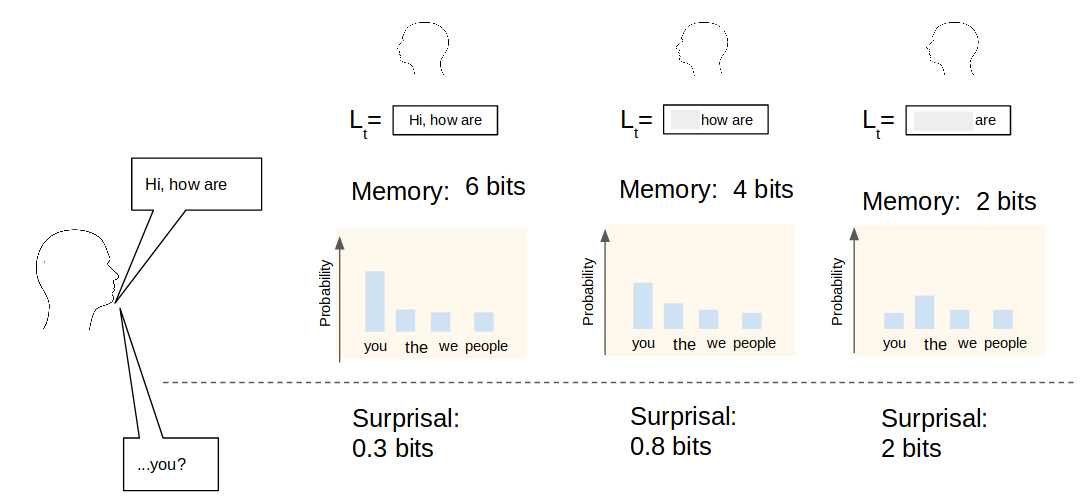
\includegraphics[width=0.9\textwidth]{figures-gdrive/communication.png}
	\caption{Memory and language comprehension. (1) A speaker produces a sequence of words. (2) A listener maintains a representation of the words received so far. The listener can represent these at higher (left) or lower (right) levels of precision. (3) Throughout communication, the listener generates probabilistic expectations about the next word. Higher precision of memory representations leads to more precise predictions. (4) When receiving the next word, the listener incurs surprisal depending on the predictions. Higher levels of fidelity in memory lead to lower surprisal on average. \jd{what do the numbers (1) (2) etc refer to? also: image is blurry, at least on my screen}\note{make reference to $L_t$ inside the caption. you and the surprisals visually better aligned. maybe can color-code? } \mhahn{problem suggests that memory has to be contiguous substrings}}
	\label{fig:communication}
\end{figure}

We begin developing our model by considering the process of language comprehension illustrated in Figure~\ref{fig:communication}, where the listener Alice is processing a stream of words uttered by an interlocutor Bob (Figure~\ref{fig:communication}). 

Experimental research has established three properties of online language comprehension, which we take as postulates:
\begin{enumerate}
\item Listeners maintain some information about the words received so far. \label{memory-postulate}
\item Listeners form probabilistic expectations about the upcoming words. \label{expectation-postulate}
\item Words are easy to process to the extent that they are predictable based on a listener's memory of words received so far. \label{linking-postulate}
\end{enumerate}
We combine these three postulates into a mathematical expression intended to summarize what is known about online language processing difficulty. Consider a listener comprehending a sequence of words $w_1, \dots, w_t, \dots, w_n$, at an arbitrary time $t$.
\begin{enumerate}
    \item Let $M$ represent the function that the listener uses to encode previous words into a memory representation, such that the listener's memory state after hearing the words $w_1, \dots, w_{t-1}$ is $m_t$ (Postulate~\ref{memory-postulate}).
    \item Let $P(w_t|m_t)$ represent the listener's subjective probability distribution at time $t$ over the next word $w_t$ (Postulate~\ref{expectation-postulate}).
    \item Then the processing difficulty associated with the word $w_t$ is proportional to the \key{surprisal} of $w_t$ given the memory state $m_t$: (Postulate~\ref{linking-postulate}):
    \begin{equation}
    \label{eq:lossy-surp}
    \text{Difficulty} \propto -\log P(w_t | m_t).\footnote{All logarithms in this work can be assumed to be to base 2.}
\end{equation}
\end{enumerate}
The claim that processing difficulty should be directly proportional to surprisal comes from \key{surprisal theory}, an established psycholinguistic theory that can capture reading time effects related to garden-path disambiguation \citep{hale2001probabilistic}, antilocality effects, and effects of syntactic construction frequency \citep{levy2008expectation}. Surprisal is a robust linear predictor of reading times in large-scale eye-tracking studies based on naturalistic text \citep{smith-effect-2013,goodkind-predictive-2018}. 

Our expression differs from the usual formulation of surprisal theory in that we consider predictability based on a (potentially lossy or noisy) memory representation $m_t$, rather than predictability based on the true complete context $w_1, \dots, w_{t-1}$. The generalization to lossy memory representations is necessary to capture empirically observed effects of memory limitations on language processing, such as dependency locality effects and structural forgetting effects \citep{futrell-noisy-context-2017,futrell2019information}.

From the perspective of information theory, surprisal measures the \key{information content} of a word $w_t$ in context. The surprisal value can be interpreted as the amount of new information contained in the word $w_t$, measured in bits, given the listener's current memory state. If processing effort is indeed proportional to surprisal, then this means that the amount of work required to process a word scales linearly with the information content of that word \citep[reflecting a general bound on the cost of computation in physical systems;][]{landau,information-engines}. 

In this work, we are interested in using theories of processing difficulty to derive predictions about languages as a whole, not about individual words or sentences. Therefore, we need a measure of the processing difficulty associated with a language as a whole. For this, we consider the \emph{average} surprisal per word in the language. We call this quantity the \key{average surprisal}, denoted $S_M$ and measured in bits: 
\begin{equation}
    \label{eq:avg-surp}
    S_M \equiv -\sum_{w_1, \dots, w_t} P(w_1, \dots, w_t) \log P(w_t | m_t) \text{ bits},
\end{equation}
where the summation $w_1, \dots, w_t$ ranges over all possible sequences of words, and the memory state $m_t$ is given by encoding the previous words $w_1, \dots, w_{t-1}$ according to the memory encoding function $M$. 

Crucially, the listener's ability to predict upcoming words accurately depends on how much she remembers about previous words. As the precision of her memory increases, the accuracy of her predictions also increases, and the average surprisal $S_M$ for each incoming word decreases. Taking an information-theoretic perspective, we can think about the amount of information (measured in bits) about previous words stored in the listener's memory state. This quantity of information is given by the \key{entropy} of the memory state, denoted $H_M$:
\begin{equation}
    H_M \equiv - \sum_m P(m) \log P(m) \text{ bits},
\end{equation}
where the summation runs over all possible memory states $m$. As the listener stores more and more bits of information about the previous words her memory state, she can achieve lower and lower surprisal values for the upcoming words. This trade-off between memory and surprisal is the main object of study in this paper.

The \key{memory--surprisal trade-off curve} answers the question: for a given amount of information about previous words $H_M$ stored in the listener's memory state, what is the lowest achievable average surprisal $S_M$? Two example trade-off curves are shown in Figure~\ref{fig:examples}. In general, as the listener stores more information about previous words in her memory state, her lowest achievable average surprisal must go down. So the curve is always monotonically decreasing. However, the precise shape of the trade-off curve depends on the structure of the language being predicted. For example, Figure~\ref{fig:examples} shows how two processes might engender different trade-off curves, with Language A allowing more favorable trade-offs than Language B. That is, for Language A, it is possible to achieve lower processing difficulty while investing less memory resources than in Language B.

Now that we have defined the memory--surprisal trade-off, we can precisely state the main hypothesis of this work:
\begin{itemize}
    \item \key{Main Hypothesis.} Natural language is characterized by a distinctively steep memory--surprisal trade-off curve.
\end{itemize}
That is, natural language is memory-efficient in the sense that it is possible to achieve a low level of processing difficulty (average surprisal $S_M$) while storing a relatively small amount of information about previous words (entropy of memory $H_M$). We will claim that the word orders of natural languages are structured to maintain memory efficiency in this sense.

In the remainder of this section, we will provide a more technical definition of the memory--surprisal trade-off curve, and then we will prove a theorem showing that more efficient memory--surprisal trade-offs are possible in languages exhibiting information locality: that is, languages where words that depend on each other are close to each other. This theorem establishes the formal link between working memory efficiency in online processing and locality in word order.

\subsection{Formal definition}

Here we provide the technical definition of the memory--surprisal trade-off curve and relate it to concepts from information theory, rate--distortion theory, and statistical complexity theory. 

Let $W$ be a stationary ergodic stochastic process generating a stream of symbols called words, indexed as $w_1, \dots, w_t$.\footnote{We will use $W$ to represent languages. Large natural language texts are neither stationary nor ergodic \citep{}. However, we are interested in explaining grammatical properties of languages, which mostly hold within sentences, not within large texts as a whole. Therefore, we will represent a language using a stochastic process consisting of repeated iid samples of sentences. This stochastic process is both stationary and ergodic.} The \key{entropy rate} of $W$ is \citep[][pp. 74--75]{cover2006elements}:
\begin{equation}
    \label{eq:entropy-rate}
    h \equiv \lim_{t \rightarrow \infty} H[w_t | w_1, \dots, w_{t-1}],
\end{equation}
where the notation $H[\cdot | \cdot]$ indicates conditional entropy \citep{cover2006elements}. The entropy rate of a stochastic process is the irreducible unpredictability of the process: the extent to which a stream of symbols remains unpredictable even given an infinite amount of information about context. Because $W$ is stationary and ergodic by construction, the limit in Eq.~\ref{eq:entropy-rate} is guaranteed to converge to a positive number. The entropy rate of natural language text has been studied by \citet{shannon1951}, \citet{takahira}, and \citet{bentz}. 

Let $M$ be a memory encoding function, i.e. a function from a sequence of words to a memory state, taking in a sequence labeled $w_1, \dots, w_{t-1}$ and outputting a memory state labeled $m_t$. The \key{average surprisal} of the process $W$ given the memory encoding function $M$ is
\begin{equation}
    S_M &\equiv \lim_{t \rightarrow \infty} H[w_t | m_t].
\end{equation}
The average surprisal $S_M$ can also be called a \key{cross entropy rate} because it measures the entropy of the process $W$ conditional not on the previously-generated symbols, but on a memory representation of those symbols. If the memory state $m_t$ stores all information about the previous words $w_1, \dots, w_{t-1}$, then $S_M = h$. Therefore, by analogy with $S_M$, we also write the entropy rate $h$ as $S_\infty$, indicating that it is the lowest average surprisal that could be attained by a listener who remembers an unbounded amount of information about previous words.

The average amount of information stored in the memory states $m_t$ is the entropy of the stationary distribution over memory states, $H_M$:
\begin{equation}
    \label{eq:memory-entropy}
    H_M \equiv H[m_t].
\end{equation}
The minimum value of $H_M$ that achieves $S_M = S_\infty$ is called the \key{statistical complexity} of the process $W$. In that case, the memory encoding function $M$ gives the \key{causal states} or \key{epsilon-machine} of the stochastic process \citep{feldman-measures-1998}. The statistical complexity of natural language has been studied by \citet{hahn2019neural}. Note that $H_M$ is not guaranteed to be finite in general. We will be imposing bounds on $H_M$ and studying the resulting values of $S_M$. 

Because the memory state $m_t$ is a function of the previous words $w_1, \dots, w_{t-1}$, we have by the Data Processing Inequality \citep[][pp. 34--35]{cover2006elements}:
\begin{equation}
    S_\infty \le S_M,
\end{equation}
and therefore we can write the average surprisal $S_M$ as a sum of two positive terms,
\begin{equation}
    S_M = S_\infty + d_M,
\end{equation}
where $d_M$ is \key{memory distortion}: the extra surprisal incurred in addition to the unavoidable surprisal $S_\infty$, owing to the lossiness of the memory encoding function $M$. 
The memory distortion $d_M$ is a KL divergence:
\begin{equation}
    \label{eq:memory-distortion}
    d_M = \lim_{t \rightarrow \infty} D_{\text{KL}} [ p(w_t | w_1, \dots, w_{t-1}) || p(w_t | m_t)].
\end{equation}
Note that the limit in Eq.~\ref{eq:memory-distortion} is not guaranteed to converge. 
Because the surprisal indicated by $S_\infty$ is not a function of the memory encoding function $M$, finding a memory encoding function $M$ to minimize $S_M$ is equivalent to minimizing the memory distortion $d_M$.

The \key{memory--surprisal trade-off curve} for a process $W$ is defined as the lowest achievable average surprisal $S_M$ for each value of $H_M$. Let $R$ denote an upper bound on the memory entropy $H_M$; then the memory--surprisal trade-off curve is given by
\begin{equation}
    \label{eq:ms-formal}
    D(R) \equiv \min_{M : H_M \le R} S_M.
\end{equation}

The memory--surprisal trade-off curve in Eq.~\ref{eq:ms-formal} is similar in form to a rate--distortion function from the theory of lossy data compression \citep[][pp. 301--347]{cover2006elements}. It differs from a typical rate--distortion problem in that rate--distortion theory typically involves finding a minimum ... 

- TODO relation to rate--distortion
- TODO relation to predictive information bottleneck



\subsection{Information locality}

The shape of the memory--surprisal trade-off is determined in part by the grammatical structure of a language, and in particular its word order:
some languages enable more efficient trade-offs than others by forcing a listener to store more bits in memory to achieve the same level of average surprisal.

Here, we will demonstrate that the memory--surprisal trade-off is optimized by word orders exhibiting \key{information locality}: that is, word orders where words that depend on each other statistically are located close to each other in time. We will argue that information locality generalizes the well-known word order principle of dependency locality, which has been studied in psycholinguistics, corpus linguistics, and typology for decades \citep{rijkhoff-word-1986,hawkins-performance-1994,gibson-linguistic-1998,liu-dependency-2018,futrell-large-scale-2015,liu-dependency-2017,temperley-minimizing-2018}. 

We will make our argument by defining a lower bound on the memory--surprisal trade-off curve (Eq.~\ref{eq:ms-formal}). This lower bound represents an unavoidable cost associated with a certain level of memory usage $H_M$; the true average surprisal $S_M$ might be higher than this bound. 

Our argument will make use of a quantity called \key{mutual information}. Mutual information is the most general measure of statistical association between two random variables. The mutual information between two random variables $X$ and $Y$, conditional on a third random variable $Z$, is defined as:
\begin{align}
    I[X:Y|Z] &\equiv \sum_{x,y,z} P(x,y,z) \log \frac{P(x,y|z)}{P(x|z)P(y|z)} \text{ bits} \\
    &= H[X|Z] - H[X|Y,Z] \\
    &= H[Y|Z] - H[Y|X,Z].
\end{align}
Mutual information is always non-negative. It is zero when $X$ and $Y$ are conditionally independent given $Z$, and positive whenever $X$ gives any information that makes the value of $Y$ more predictable, or vice versa. 

We will study the mutual information structure of natural language sentences, and in particular the mutual information between words at certain distances in linear order. Define $I_t$ as the mutual information between words at distance $t$ from each other, conditional on the intervening words:
\begin{align}
    I_t &\equiv I[w_t : w_0 | w_1, \dots, w_{t-1}] \\
    &= H[w_t | w_1, \dots, w_{t-1}] - H[w_t | w_0, \dots, w_{t-1}].
\end{align}
This quantity, visualized in Figure~\ref{fig:theorem} (a), measures how much predictive information is provided about a given word by the word $t$ steps in the past.
It is a statistical property of the language, and can be estimated from large-scale text data.

Equipped with this notion of mutual information at a distance, we can now state our theorem:
\begin{thm}\label{prop:suboptimal}(Information locality) For any positive integer $T$, consider a memory encoding function $M$ such that
\begin{equation}
\label{eq:memory-bound}
H_M \le \sum_{t=0}^T t I_t.    
\end{equation}
Then we have a lower bound on the average surprisal under the memory encoding function $M$:
\begin{equation}
\label{eq:surprisal-bound}
S_M \ge S_\infty + \sum_{t=T}^\infty I_t.
\end{equation}
%Let $T$ be a positive integer, and consider a listener using at most $\sum_{t=1}^T t \operatorname{I}_t$ bits of memory on average.
%Then this listener will incur average surprisal at least
%$\operatorname{H}[w_t|w_{<t}] + \sum_{t > T} \operatorname{I}_t$.
\end{thm}
A formal proof, relying only on the stationarity of the stochastic process, is given in Appendix Section X. 

The meaning of the theorem is illustrated visually in Figure~\ref{fig:theorem}. The theorem describes a memory encoding function which remembers all relevant information from $T$ words in the immediate past and forgets all information from words beyond $T$ timesteps into the past. The memory requirements for such a memory encoding function are at least $\sum_{t=0}^T t I_t$ (Eq.~\ref{eq:memory-bound}), reflecting the cost of holding $I_t$ bits in memory for $t$ timesteps. This memory encoding function forms a $T$th-order Markov approximation to the stochastic process. The surprisal cost for this memory encoding function is at least $\sum_{t=T}^\infty I_t$ (Eq.~\ref{eq:surprisal-bound}), which is the sum of all the predictive information contained in words more than $T$ timesteps in the past, which was forgotten by the memory state (see Figure~\ref{fig:theorem}(b)). The theorem states that this procedure gives a lower bound on the memory--surprisal trade-off curve, meaning that there is no memory encoding function with memory entropy $H_M$ which achieves lower average surprisal than Eq.~\ref{eq:surprisal-bound}.




% THINK ABOUT THIS: The actual memory requirements of the T'th order Markov approximation might be higher than H_M because H_t > I_t.


%Here we propose to model human language comprehension by treating the listener's memory $m_{i-1}$ as a lossily compressed representation of the context $x_{1...i-1}$, and the processing effort associated with each word using Eq.~\ref{eq:lossy-surp}.
%Suppose that the listener's memory has a fixed information-carrying capacity $k$, then this listener has to compress the context into a memory representation $m_{i-1}$ with at most $k$ bits: $H[m_{i-1}] \leq k$.
%Information theory implies that the processing cost $S_M$ trades off with the memory capacity $k$:
%Processing cost will be lower for a listener who represents past input at higher levels of precision.




%We prove a theorem describing how the shape of this tradeoff relates to language structure. %relating memory to the experienced comprehension difficulty $S$.
%Informally, the theorem says that languages support more efficient tradeoffs between short-term memory and comprehension difficulty when words are strongly predictive of their neighboring words.
%This theorem captures formally that languages support more efficient tradeoffs between short-term memory and comprehension difficulty when words are strongly predictive of their neighboring words.


%We derive the precise form of the memory-surprisal tradeoff in Theorem 1.
%Let $\operatorname{I}_t$ be the conditional mutual information between words that are $t$ steps apart, conditioned on the intervening words: 
%\begin{equation}%
%	\operatorname{I}_t := \operatorname{I}[w_t, w_0 | w_1, \dots, w_{t-1}] = \operatorname{H}[w_t|w_1, \dots, w_{t-1}] - \operatorname{H}[w_t|w_0, \dots, w_{t-1}] 
%\end{equation}

%This quantity measures how much predictive information the word $t$ steps in the past contains about the current word, above and beyond the information contained in the intervening words.

%This is equal to the reduction in uncertainty about the $t$-th observation when %knowing the $0$-th observation, in addition to the block of intervening observations.
%That is, we measure the amount of statistical dependency of observations that are $t$ steps apart, controlling for any information that is redundant with intervening observations.
%This quantifies how much information needs to be carried across $t$ timesteps without any possibility for `guessing' it from intervening observations.




Our theoretical results describe how the tradeoff between memory and comprehension difficulty relates to $I_t$ (Figure~\ref{fig:theorem} (b)):
Consider a listener who invests $B$ bits of memory into representing past input.
We then consider the smallest $T$ such that the area under the curve of $t I_t$, to the left of $T$, has size $B$.
Such a listener will experience average surprisal at least $H[w_t| w_{<t}] + \sum_{t=T+1}^\infty I_t$. %\note{maybe result first, and then say what $T$ is}
By tracing out all values $T >0$, one can obtain a bound on the tradeoff curve for any possible listener.

%This is formalized in the following theorem:

%\begin{thm}\label{prop:suboptimal}
%Let $T$ be a positive integer, and consider a listener using at most $\sum_{t=1}^T t \operatorname{I}_t$ bits of memory on average.
%Then this listener will incur average surprisal at least
%$\operatorname{H}[w_t|w_{<t}] + \sum_{t > T} \operatorname{I}_t$.
%\end{thm}






The theorem gives us a lower bound on the listener's memory-surprisal curve: Taking all pairs of memory $\sum_{t=1}^T t I_t$ and surprisal $H[w_t|w_{<t}] + \sum_{t > T} I_t$.
Then interplate linearly (justify this in appendix).
We obtain a curve in memry-surprisal plane, which is a lower bound on the memory demands of any listener at a given surprisal level.
We visualize this for the two processes from Figure~\ref{fig:basic} in Figure~\ref{fig:listener-tradeoff}.



\paragraph{Mathematical Assumptions}
Here we make explicit which formal assumptions go into the theoretical result.

\begin{enumerate}
\item Ingredient 1: Language as a Stationary Stochastic Process:
We represent language as a stochastic process of words $\dots w_{-2} w_{-1} w_0 w_{1} w_{2} \dots$, extending indefinitely both into the past and into the future.
The symbols $w_i$ belong to a common set, representing the words of the language.\footnote{Could also be phonemes, sentences, ..., any other kind of unit.}

The assumption of infinite length is for mathematical convenience and does not affect the substance of our results:
As we restrict our attention to the processing of individual sentences, which have finite length, we will actually not make use of long-range and infinite contexts.

We make the assumption that this process is \emph{stationary}.
Formally, this means that the conditional distribution $P(w_t|w_{<t})$ does not depend on $t$, it only depends on the actual sequence $w_{<t}$.
Informally, this says that the process has no `internal clock', and that the statistical rules of the language do not change at the timescale we are interested in.
In reality, the statistical rules of language do change: They change as language changes over generations, and they also change between different situations -- e.g., depending on the interlocutor at a given point in time.
Given that we are interested in memory needs in the processing of \emph{individual sentences}, at a timescale of seconds or minutes, stationarity seems to be a reasonable assumption to make.

\item Ingredient 2: Flow of Information: There are no assumptions about the memory architecture and the nature of its computations.
However, we make a basic assumption about the flow of information (Figure~\ref{fig:listener-markov}):
At a given point in time, the listener's memory state $m_t$ is determined by the last word $w_t$, and the prior memory state $m_{t-1}$.
As a consequence, $m_t$ contains no information about the utterances beyond what is contained in the last word observed $w_{t-1}$ and in the memory state before that word was observed $m_{t-1}$.
As a consequence, the listener has no knowledge of the speaker's state beyond the information provided in their prior communication.
This is a simplification, as the listener could obtain information about the speaker from other sources, such as their common environment (weather, ...).
See Section XX for further discussion.
\end{enumerate}


\paragraph{Informal Argument}
An intuitive (non-rigorous) argument for this theorem goes as follows:
For each bit of information that is held in memory, we count the number of timesteps from when it is first entered into memory to when it is forgotten.
If a word $w_{T-t}$, $t$ steps in the past, contains one bit of information about the current word $w_T$, and if this information is not redundant with information in the intervening words, then this bit of information had to be maintained in memory for $t$ steps.
The amount of such information is $I_t$. This explains the factor $t$.


\paragraph{Discussion}
The theorem allows us to estimate the extra surprisal associated with each amount of memory capacity for a language.
The quantities $\operatorname{I}_t$ can be estimated as the difference between the cross-entropy of language models that have access to the last $t-1$ or $t$ words.
Given such estimates of $\operatorname{I}_t$, we estimate tradeoff curves as in Figure~\ref{fig:tradeoff} by tracing out $T=1, 2, \dots$.


Our result is entirely information-theoretic and applies to \emph{any} physical encoding of the past, entirely independent of the implementation of the model. % and the mechanisms by which it computes predictions.
In particular, while the relation to psycholinguistic and psychological models of how memory works will be interesting to explore (see Section X), our result applies to any such model.
Memory representations do not have to be rational or optimal for this bound to hold:
It provides a \emph{lower bound} on the amount of information that needs to be stored -- other memory representations will always need to store at least as much information.



There are theories of retrieval where the main bottleneck lies not in capacity, but in difficulty of retrieval. See General Discussion for an extension of our analysis that applies to such models.




\begin{figure}
	(a)
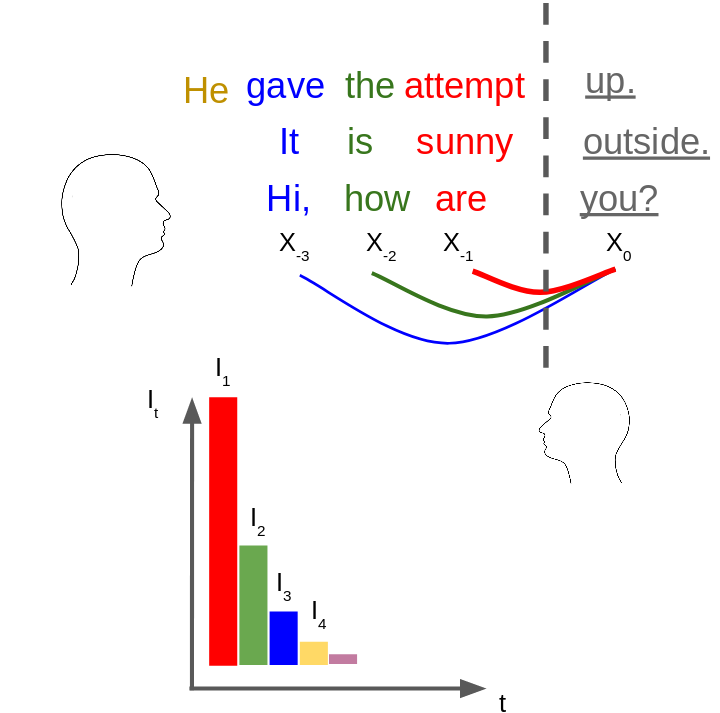
\includegraphics[width=0.4\textwidth]{figures-gdrive/mi-distance.png}
	(b)
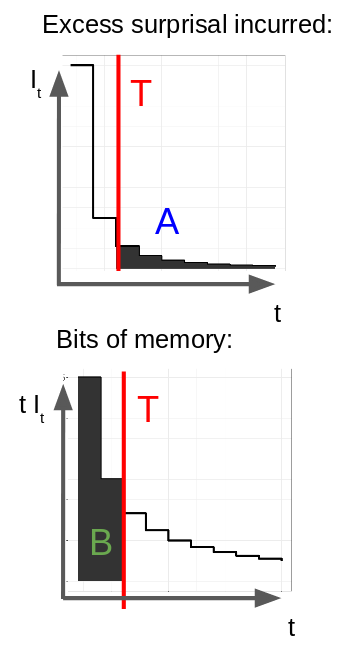
\includegraphics[width=0.2\textwidth]{figures-gdrive/theorem.png}
	(c)
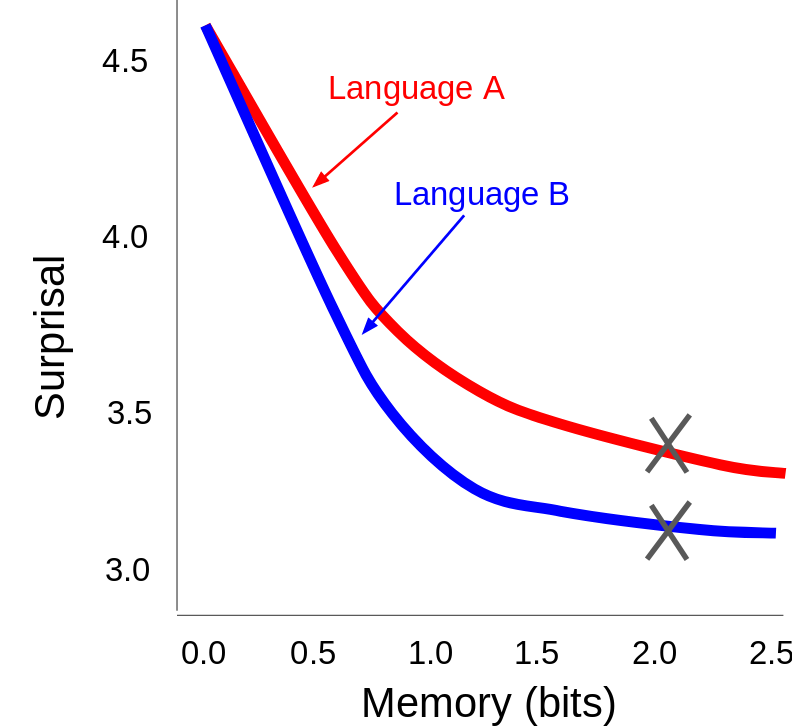
\includegraphics[width=0.2\textwidth]{figures-gdrive/tradeoff.png}
	\caption{
		(a) Conditional mutual information $I_t$ captures how much predictive information about the next word is provided, on average, by the word $t$ steps in the past.
		(b) Here we illustrate our theoretical result. We plot $I_t$ (top) and $tI_t$ (bottom) as functions of $t$. A listener using $B$ bits memory (bottom) to represent prior observations will incur at least $A$ bits of extra surprisal beyond the entropy rate (top). \note{there is t and T. COnfusing}
		(c) \jd{FILL OUT} \note{make the colors in (c) difefrenfr from this in (b). Do want to make clear what the mapping from (b) to (c) is. Maybe can even have a pair of the two (b) curves, and then show what they map on.}
}\label{fig:theorem}
\end{figure}







%\begin{figure}
%	\begin{center}
%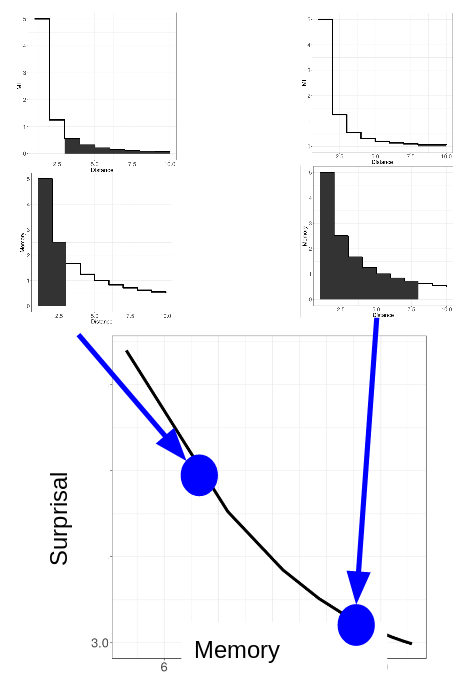
\includegraphics[width=0.45\textwidth]{figures/interpolate-curve.png}
%\end{center}
%	\caption{Estimating memory-surprisal tradeoff using the Theorem: We trace out the memory and surprisal values for all $T=1, 2, ...$, and linearly interpolate the curve.}\label{fig:interpolate}
%\end{figure}




%\begin{figure}
%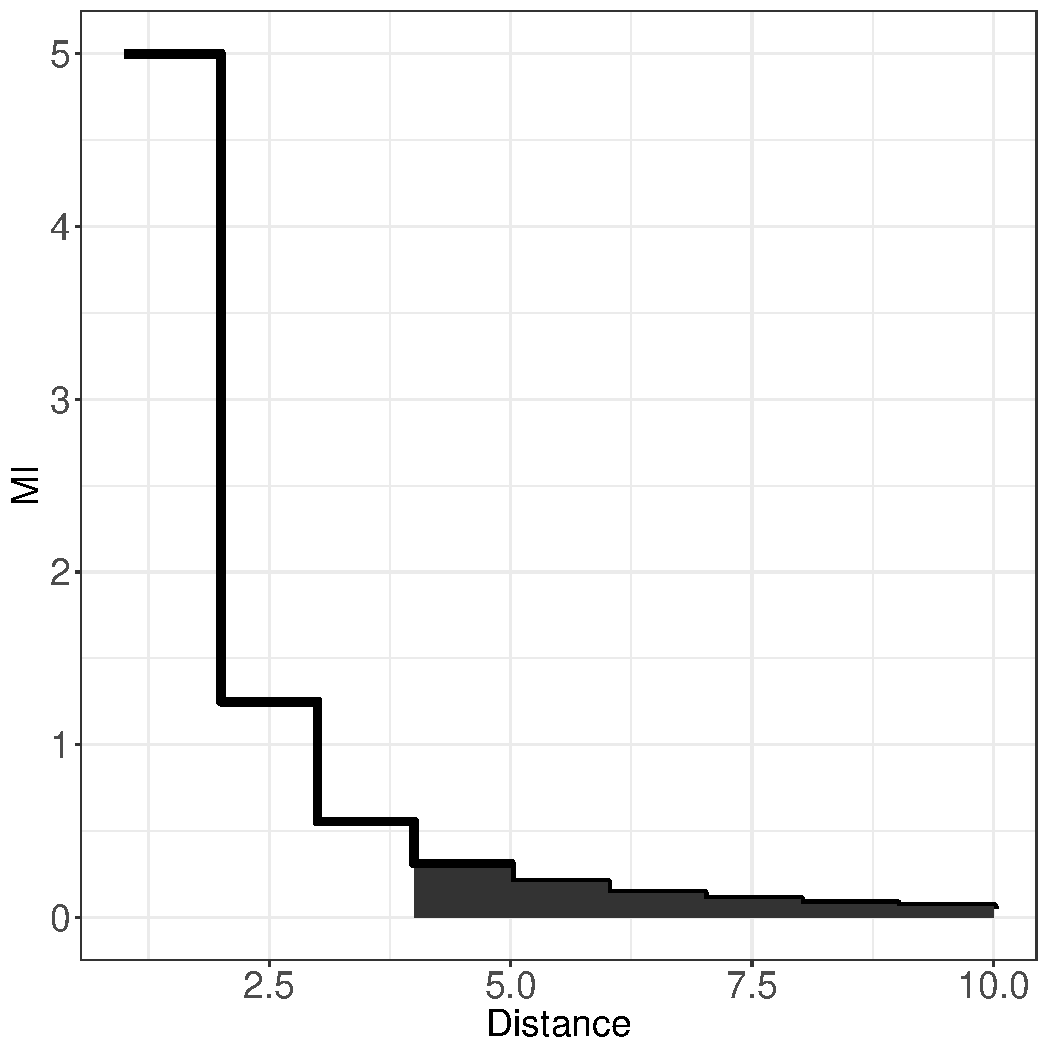
\includegraphics[width=0.45\textwidth]{figures/add-surp.pdf}
%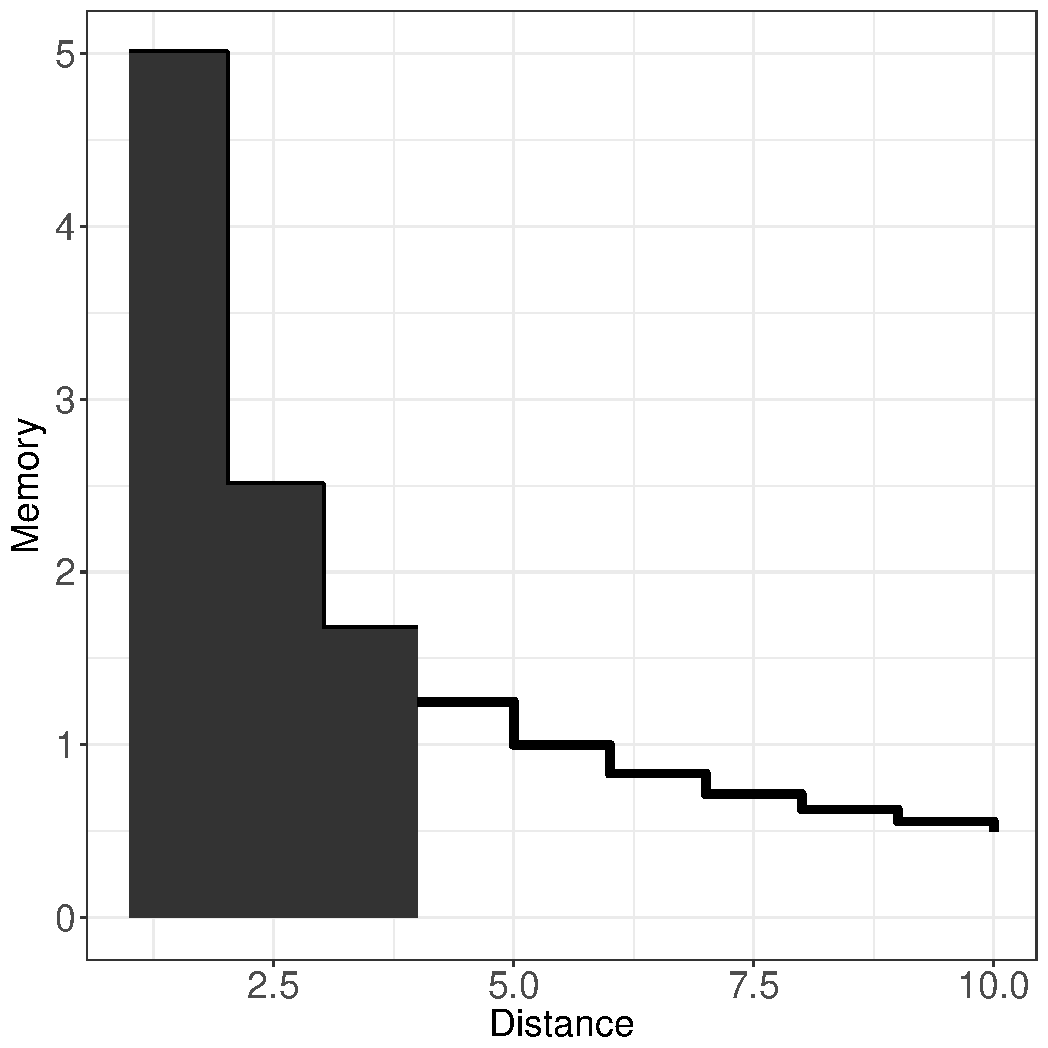
\includegraphics[width=0.45\textwidth]{figures/lower-mem.pdf}
%	\caption{Illustration for Proposition~\ref{prop:suboptimal}. Listeners can trade off memory and surprisal: A listener only investing memory of the amount given by the black area on the right will incur at least the black area on the left in additional surprisal. In the given example, $T=4$. By varying $T$, the two areas describe the listener's memory-surprisal tradeoff curve.}\label{fig:listener-tradeoff-decay}
%\end{figure}





%\subsection{Formal Analysis and Proofs}






\paragraph{Consequence: Information Locality} %\label{sec:info-locality}

Due to the factor $t$ inside each term of the sum, carrying the same amount of information over longer distances requires more memory -- that is, modeling long statistical dependencies is more costly in terms of memory than modeling shorter ones.
This formalizes a general link between memory and locality in language production.
In Section~\ref{sec:listener}, we will extend this analysis to listeners performing incremental prediction.

The proposition implies that memory is decreased if $I_t$ decreases quickly as $t \rightarrow \infty$ -- that is, if the contributions of long-term dependencies in the process are small.

We illustrate Proposition~\ref{prop:lower-bound} in Figure~\ref{fig:basic}.
We consider two processes A and B, where $I_t := 5t^{-1.5}$ for $A$ and $I_t := 3.5 t^{-2.5}$ for $B$.
The curves of $I_t$, as a function of the distance $t$, are shown in Figure~\ref{fig:basic} (left).
In both cases, $I_t$ converges to zero as $t$ grows to infinity. 
However, $I_t$ decays more quickly for Process A (red).
This means that predictive information about an observation is concentrated more strongly in the recent past.
In Figure~\ref{fig:basic} (right), we show $t\cdot I_t$ as a function of $t$.
Note that the area under the curve is equal to (\ref{eq:memory-bound}).
This area is smaller for the red process, as $I_t$ decays more quickly there.  



\begin{figure*}
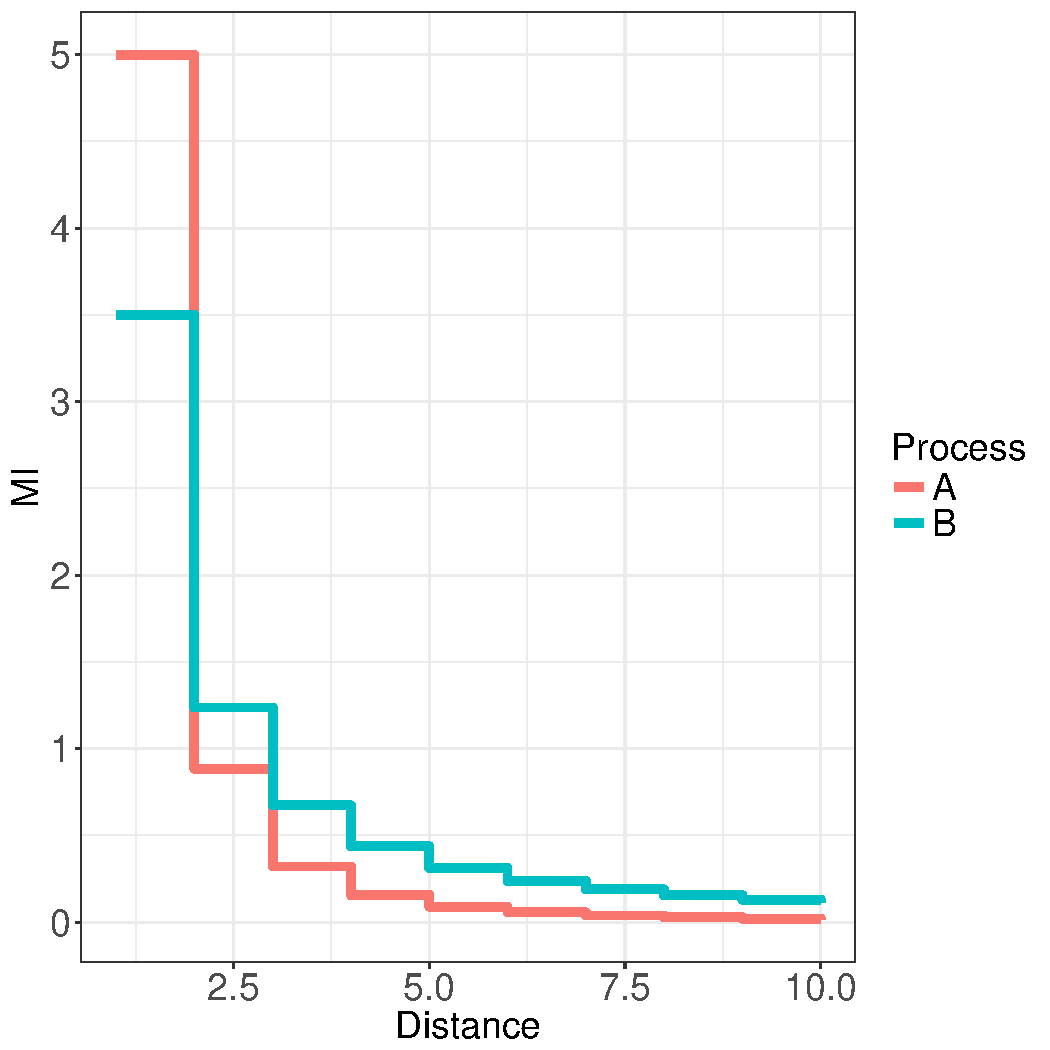
\includegraphics[width=0.45\textwidth]{figures/decay.pdf}
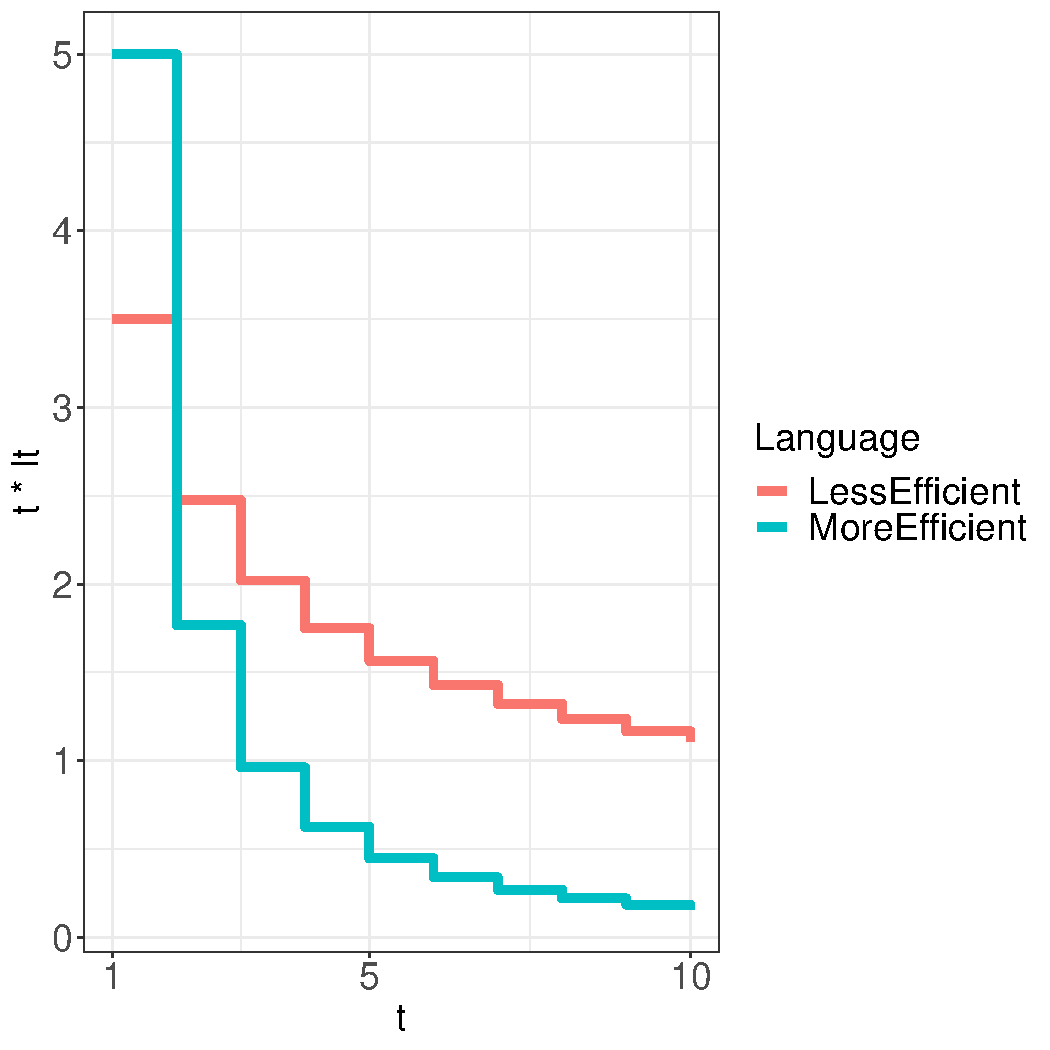
\includegraphics[width=0.45\textwidth]{figures/memory.pdf}
%
	\caption{Left: $I_t$ as a function of $t$, for two different processes. $I_t$ decays faster for the red process: Predictive information about the present observation is concentrated more strongly in the recent past. Left: $t \cdot I_t$ as a function of $t$ for the same processes. }\label{fig:basic}
\end{figure*}

\begin{figure}
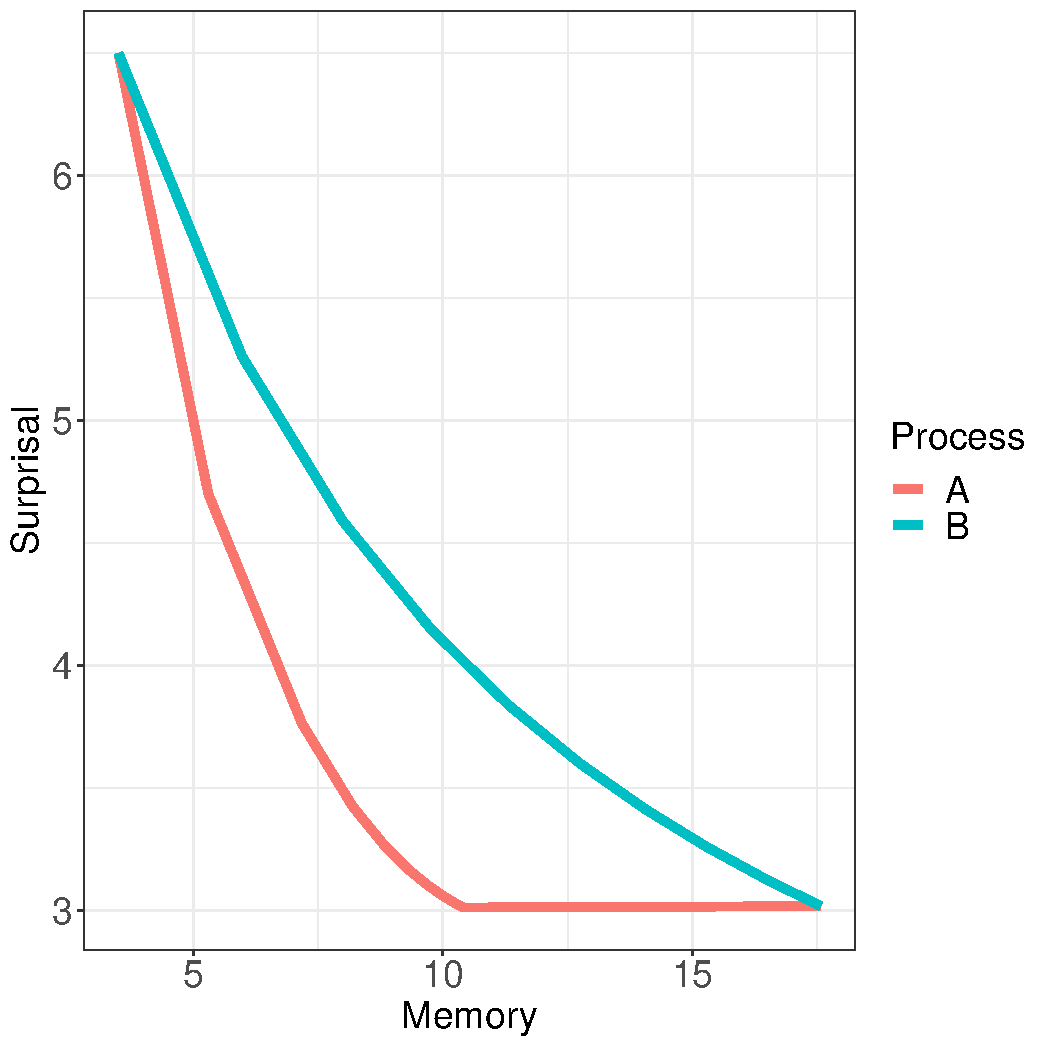
\includegraphics[width=0.45\textwidth]{figures/listener-tradeoff.pdf}
	\caption{Listener's memory-surprisal tradeoff for the two processes in Figure~\ref{fig:basic}. Recall that the red process had a faster decay of conditional mutual information. Correspondingly, this figure shows that a listener can achieve lower surprisal at the same level of memory load.}\label{fig:listener-tradeoff}
\end{figure}



\subsubsection{Relation to Dependency Locality}



